\cotefile{74}
\scanpage{38}
Pour tte application
\[
z_{\rho}\colon V\mathbin{\unsure{-|\to}}Z
\]
de $V$ dans un groupe commutatif, $Z$,
satisfaisant les deux relations précédentes,
$\exists$ une extension $\widetilde{\Gamma}^{(z_\rho)}$ de $\Gamma$ par $Z$,
et des $\psi_i^{(z_\rho)}$ relevant les $\varphi_i$, donnant
naissance (via $\rho$) à $z_\rho$, et
le système de cette extension et
des $\psi_i$ ($i\in I$) est déterminée à isom
unique près.

Il y a un $Z$ ``universel'' $\unsure{\mathfrak Z|\mathscr Z}_{V\deleted{\unsure{,\rho}}}$
savoir le quotient de $\mathbb Z^{(V)}$ par
les ``relations'' précédentes.\textsuperscript{\ensuremath{\diagup\mkern-6mu\backslash}}
% margin note written sideways
\margin{\ensuremath{\diagup\mkern-6mu\backslash}\ Il \unsure{apparait|apparaît} comme noyau d'une ext. universelle $\widetilde{\Gamma}$ de $\Gamma$ qu'une fois choisi $\rho$. Le noyau (\unsure{indépendt|indépendant|bi-dépendt|indépendamment} du choix d'un $\rho$ \unsure{pour|possibles}) est alors $\mathfrak Z^{\unsure{\mathrm{or}|\omega}}=\mathfrak Z\wedge_{\pm1}\mathrm{or}$, \deleted{\unsure{on}} $z_\rho\colon V-\mathfrak Z^{\mathrm{or}}$ par $z_\rho(x)=\deleted{\unsure{z}}\,(x\wedge\rho)$, \unsure{où|i.e.} $\lambda\colon V-\mathfrak Z$ est l'appl. can. et on aura bien \( \begin{aligned} z_{\bar\rho}(x)&=\lambda(x\wedge\bar\rho)=\lambda(-x\wedge\rho)\\ &=-\lambda(x\wedge\rho)=-z_\rho(x) \end{aligned} \) i.e. $z_{\bar\rho}(x)=-z_\rho(x)$ \ldots.}
Notons que si $z_\rho$ est \deleted{\unsure{donc}} un \unsure{hom|hom.} de groupe
resp. une application $2$-quadratique, les
conditions \unsure{$\infty$|st|$\circ$|sont} satisfaites, ce qui
montre que $\mathfrak Z_V$ contient comme
% archive sheet number: 37
\scanpage{39}
\deleted{\unsure{le}} quotient \textsuperscript{\ensuremath{\diagup\mkern-6mu\backslash}}
% slanted
\margin{\ensuremath{\diagup\mkern-6mu\backslash}\ un sous-groupe de \ldots. savoir celui engendré par les $x+x^{(2)}$ $(x\in V)$}
la somme $V+\Gamma^2_{\mathbb Z}(V)$
(qui est le $\mathbb Z$-module universel qui
reçoit $V$ par une application pol. de
degré $\leq2$ sans terme constant).

\begin{center}\rule{1.3cm}{0.35pt}\end{center}

\uline{Ex} $V$ est un vectoriel \deleted{de dim $2$} sur $\mathbb F_2$.

\deleted{Soit $J=V^{*}=V\smallsetminus\{0\}$, la donnée de $V$ équivaut à celle de l'ens $J$ de card $3$. On a}
\[
\deleted{\mathfrak Z=\mathbb Z^{(J)}\big/\text{relations }\unsure{\mathrm{or}|\infty}}
\]

Dans ce cas, on \deleted{\unsure{prouve|puisque}} \inserted{voit} que \unsure{tte|toute} application $\lambda\colon V\longrightarrow Z$ telle que
\[
\deleted{\unsure{\star}}\qquad
\lambda(x+y)-\lambda(x)-\lambda(y)=\mu(x,y)
\quad\text{(\unsure{fonction|fonct.} $2$-bil. sym)}
\tag*{H)}
\]
\figure{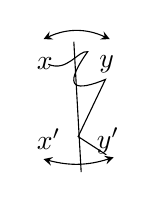
\begin{tikzpicture}[x=.55cm,y=.55cm,>=stealth]
\draw[<->] (-.75,1.65) to[bend left=25] (.78,1.65);
\draw[<->] (-.75,-1.12) to[bend right=16] (.87,-1.08);
\draw (-.05,1.59)--(.12,-1.42);
\draw (-.64,1.07) .. controls (-.2,.88) and (.05,1.4) .. (.27,1.36) .. controls (-.36,.47) and (.02,.45) .. (.68,.72) -- (.05,-.6) -- (.70,-1.02);
\node at (-.72,1.09) {$x$}; \node at (.71,1.08) {$y$};
\node at (-.63,-.65) {$x'$}; \node at (.74,-.70) {$y'$};
\end{tikzpicture}}
est polynomiale (en effet, on aura $\lambda(0)=0\overset{\text{d'où}}{\Longrightarrow}$
$\lambda(\underset{\inserted{\substack{\shortparallel\\0}}}{2x})=2\lambda(x)+\mu(x,x)$, donc $\mu(x,x)=-2\lambda(x)$ \deleted{donc}
$\mu(x,x)\in2Z$ $(\forall x\in V)$, d'où \unsure{facilemt|facilmt|facilement} le
résultat). Donc
\[
\unsure{\mathfrak Z|\mathscr Z}\mathrel{\unsure{=|\subset}} V+
\underset{\displaystyle
 (\mathbb Z/4\mathbb Z)^{(I)}\deleted{+\mathbb Z/4\mathbb Z}
 +(\mathbb Z/2\mathbb Z)^{\mathcal P_2(I)}}{\underbrace{\Gamma_{\mathbb Z}^2(V)}}\unsure{\searrow|\shortparallel}
\]

\hfill TSVP
% archive sheet number: 38
\scanpage{40}
Supposons que $V$ soit de dim \unsure{$2$} \inserted{sur $\mathbb F_2$}. Alors
il y a une forme quadratique
canonique sur $V$, définie par
\[
q(x)=\begin{cases}0&\text{si }x=0\\1&\text{si }x\ne0\end{cases}
\]
qui \unsure{donné|donne} donc lieu à une ext.
centrale canonique de $\Gamma(V)$ par $\mathbb Z/2\mathbb Z\simeq\mathbb F_2$
telle que
\[
\begin{aligned}
\unsure{\varphi|\psi}_{i_0}(x)\varphi_{i_1}(x)\varphi_{i_2}(x)&=z
\quad\text{(él. non nul de}\\[-2pt]
&\hspace{4.8em}Z=\mathbb Z/2\mathbb Z\text{)}
\end{aligned}
\]
$\forall x\in V^{\omega}$ (et un \deleted{\unsure{pour tout ordre|ordre circulaire}} \inserted{ordre \unsure{total|fixé|triplet} $(i_0,i_1,i_2)$}
sur $I$ \ldots)
% archive sheet number: 39
\scanpage{42}
\diagram{\(\setlength{\arraycolsep}{2pt}\begin{array}{c|c||c||l|l|l}
\multicolumn{2}{c||}{\text{\unsure{Sohier|Sophie|Sohie}}}&\text{\unsure{Eu|Ens|Eve}}&&
\text{Agnès, réserve}&\text{\unsure{cire|Cire}}\\ \hline
\deleted{\unsure{20}}\,15&10&&30\quad30\;(\text{ou }\unsure{25|20})&
12,\deleted{\unsure{10}}\,\inserted{8},5\deleted{\unsure{1}},3&\\
\deleted{\unsure{4}}\,5&5\;5&5&
3,3,3,3\quad\text{(j'ai }30,10,10,5\text{)}&&\cdot\\
3\;3\;3&&&&&
\end{array}\)}

\diagram{\(\begin{array}{rcl}
2&\text{à}&\unsure{25|26}\ \text{ou }30\\
1&\text{à}&15\\
2&\text{à}&10\\
5&\text{à}&5\\
8&\text{à}&3
\end{array}\)}
\diagram{\(\begin{array}{|rcl@{\quad}c|r|}
\hline
2&\text{à}&\unsure{22|27}\ \text{ou }30&\deleted{\unsure{7}}&250\\
1&\text{à}&\unsure{17|15}&&60\\ \cline{1-1}
1&\text{à}&13&&45\\
1&\text{à}&10&&37\\ \cline{1-1}
1&\text{à}&8&&30\\
5&\text{à}&5&&140\\ \cline{1-1}
\multicolumn{3}{|c}{\left.\begin{array}{rcl}\unsure{2|7}&\text{à}&4\\6&\text{à}&3\end{array}\right\}}&&200\\ \hline
\multicolumn{4}{c|}{}&760\\ \cline{5-5}
\end{array}\)}
\diagram{\(\begin{array}{c|r|r}
\deleted{\unsure{3}}&&\\ \hline
4&17{,}80&5{,}40\\
5&21{,}60&6{,}50\\
6&25{,}20&7{,}00\\
7&34{,}20&8{,}80\\
8&45{,}\text{--}&9{,}20\\ \hline
\end{array}\)}

Vidal (\unsure{Chrysalia|Chrysalia.})\\
\unsure{Ala|Aba}\\
Boite Postale 72\\
11000 Carcassonne\\
Tel: 47 82 44

% The following lines are inverted relative to the tables.
$E$ ens à $5$ él, on va lui associer \unsure{canoniqmt|canoniquemt|canoniquement} un
dodécaèdre combinatoire (d'où un icosaèdre
combinatoire)

$F={}$ ens des faces $={}$ ens des $12$ structures polygonales sur $E$

Le polygone combinatoire associé
% archive sheet number: 41
\scanpage{43}
\mspage{(29)}
% archive sheet number: 42
\scanpage{44}
petits clous\\
\unsure{percer|pince|perceur|pour} \unsure{baguette|baguettes}\\
planchette

\figure{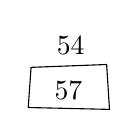
\begin{tikzpicture}[x=.6cm,y=.6cm]
\draw (0,0)--(.06,.85)--(1.66,.91)--(1.72,-.04)--(0,0);
\node[above] at (.9,.91) {$54$};
\node[above] at (.85,-.04) {$57$};
\end{tikzpicture}}
\figure{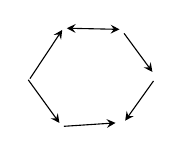
\begin{tikzpicture}[x=.72cm,y=.72cm,>=stealth]
\draw[->] (-1.1,0)--(-.53,.86); \draw[<->] (-.45,.89)--(.48,.87);
\draw[->] (.56,.8)--(1.06,.12); \draw[->] (1.08,-.04)--(.58,-.74);
\draw[->] (-.5,-.84)--(.41,-.78); \draw[->] (-1.13,-.02)--(-.58,-.78);
\end{tikzpicture}}
\figure{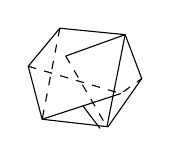
\begin{tikzpicture}[scale=.68]
\draw (-1.08,.27)--(-.49,.98)--(.73,.86)--(1.04,.04)--(.41,-.86)--(-.82,-.72)--cycle;
\draw (-.82,-.72)--(.65,-.24) (.73,.86)--(-.38,.46) (.73,.86)--(.39,-.86) (-.06,-.47)--(.26,-.89);
\draw[dashed] (-.49,.98)--(-.82,-.72) (-1.08,.27)--(.65,-.24)--(1.04,.04) (-.38,.46)--(.39,-.86);
\end{tikzpicture}}

\[
\begin{aligned}
 S&=\tau\times\varepsilon
 &\widetilde S&=\tau\times\varepsilon\times\omega(\tau)\\
 A&=\tau\times(\varepsilon\wedge\omega(\tau))
 &&\tau\times\varepsilon\mathbin{\cdot}\tau\times\varepsilon'\\
 &\tau\times(\varepsilon\wedge\omega(\tau))\wedge\omega(\unsure{\prime|\,|\tau'})
 &&\bigg\backslash\,(\varepsilon,\alpha)\quad(\alpha,\beta)\\
 &&&\text{\unsure{resp}}\,(\alpha\wedge\beta)\,\unsure{s|3}\\
 &&&\tau\times\varepsilon\times\varepsilon'
\end{aligned}
\]
\diagram{\begin{tikzcd}[ampersand replacement=\&,row sep=small,column sep=small]
{} \arrow[dr,dash] \& \& \tau\times\varepsilon \arrow[dl,dash] \& {(\mathrm{tri})'}^{\varepsilon} \arrow[d,"3"]\\
\& \tau \& \unsure{\mathrm{tritria}|\mathrm{tritrio}|\mathrm{Tritria}}\arrow[r,"2","{\unsure{,\cdot}}"'] \& \mathrm{Hex}\\
\& \& {} \arrow[ur] \&
\end{tikzcd}}

\margin{\unsure{$\leftarrow\!\shortmid$}}
\diagram{\begin{tikzcd}[ampersand replacement=\&,row sep=small,column sep=small]
\& R\arrow[dl]\arrow[dr] \&\\
\tau\times\varepsilon\arrow[d]\arrow[dr,"\deleted{\unsure{\times}}"] \& \& \tau\times\varepsilon'\arrow[d]\arrow[dl,"\deleted{\unsure{\wedge}}"]\\
\tau \& \deleted{\unsure{\leftrightarrow|\rightrightarrows}}\ \underset{\unsure{\mathrm{par}}}{=}\&\tau
\end{tikzcd}}
\begin{center}\deleted{\uuline{\unsure{canons|canoniq}}}\end{center}

\diagram{\begin{tikzcd}[ampersand replacement=\&,column sep=.75em,row sep=1.5em,cells={nodes={font=\scriptsize}}]
\&\&\& S\&\\
\&\&S\&\&\\
\&\&\& {\mathrm{hex}+\mathrm{diag}\simeq\unsure{\mathrm{tri.}\,\mathrm{di}}+\unsure{\varepsilon(\mathrm{dual})}}\arrow[ul]\arrow[d,"3"]\&\\
(\mathrm{tria}')\arrow[d,"3"']\&(\deleted{\unsure{\mathrm{tri}}})\arrow[l]\arrow[d]\&(\unsure{\mathrm{tri}_{*}|\mathrm{tri}|\mathrm{tria}})\arrow[l,dash]\arrow[d]\&{\simeq\mathrm{hex}}\&{\mathrm{hex}+\unsure{\mathrm{somm.}}}\arrow[ul,"2"']\arrow[uuul,bend right=32]\arrow[d,"3"]\\
\mathrm{Hex}\arrow[dd,"3"']\arrow[dr,"\unsure{\mathrm{tribus}}"']\&\deleted{\unsure{\mathrm{Tritria}}}\arrow[l,"2"]\&\unsure{\mathrm{Tritrio}|\mathrm{Tritria}}\arrow[l,dash]\&\&{(\unsure{\mathrm{trior}|\mathrm{tria}\times2})\simeq\mathrm{hex}+\substack{\text{triangle}\\\text{inscrit}}}\arrow[ul,"2"]\arrow[lll,bend right=6,dash]\arrow[d,"{\unsure{2\,\mathrm{hex}\,\acute{\mathrm ep}}}"]\\
\&{\unsure{\mathrm{Hexor}|\mathrm{Hexorien}}\simeq\unsure{\mathrm{or}|\omega}(\mathrm{tria}'/\mathrm{Hex})}\arrow[ul,"2"]\arrow[uul]\&\&\&\unsure{\mathrm{Tortria}|\mathrm{Tortrio}|\mathrm{Tritria}}\arrow[llu]\arrow[lll]\\
(\mathrm{triHex})\&\&\&\&
\end{tikzcd}}
\[
\deleted{\tau\times\varepsilon\times\omega(\tau)}
\]
\figure{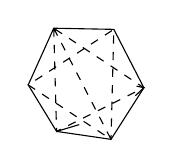
\begin{tikzpicture}[scale=.72]
\draw (-1,0)--(-.55,1)--(.51,.98)--(1.04,-.05)--(.46,-.96)--(-.5,-.82)--cycle;
\draw[dashed] (-.55,1)--(.46,-.96)--(-1,0)--(.51,.98)--(.46,-.96)
 (-.55,1)--(-.5,-.82)--(1.04,-.05)--(-.55,1);
\draw (-.5,-.82)--(-.10,-.7) (.91,-.02)--(1.04,-.05)--(.89,-.19);
\end{tikzpicture}}
% archive sheet number: 43
\scanpage{45}
\diagram{\begin{tikzcd}[ampersand replacement=\&,row sep=small,column sep=small]
\&\unsure{\zeta|s|\}}_{14}\arrow[r,dash]\arrow[dl,dash,shift left]\arrow[dl,dash,shift right]\&\zeta_{25}\arrow[dll,dash]\arrow[dr,dash]\&\deleted{\unsure{\zeta_1|\zeta_{15}}}\\
\zeta_{\unsure{35|32|34}}\arrow[dr,dash]\&\&\&\zeta_{16}\arrow[dll,dash,shift left]\arrow[dll,dash,shift right]\\
\&\zeta_{24}\arrow[uur,dash]\&\&
\end{tikzcd}}
\[
\begin{aligned}
 & &\zeta_{14}&\\
 &\zeta_{25}&&\zeta_{26}\\
 &\zeta_{16}&&\zeta_{15}\\
 &&\zeta_{24}&
\end{aligned}
\]
\figure{\begin{tikzpicture}[x=.72cm,y=.72cm]
\draw (-1.6,.05)--(.32,1.12)--(1.12,-.05)--(.30,-1.25)--(-.78,-1.16)--cycle;
\draw (-.78,-1.16)--(-.2,-.44)--(.30,-1.25) (-.8,-1.0)--(-.82,.9) (-.86,1.12)--(.32,1.12) (-.86,1.12)--(-.31,1.75)--(-.5,.86);
\node[left] at (-1.5,.09) {$\unsure{a|x_1}$}; \node[below] at (-1.42,.09) {$\unsure{=}$};
\node[left] at (-.86,1.15) {$\unsure{x|x_2}$};\node[above] at (.32,1.12) {$x_4$}; \node[right] at (.33,1.12) {$=\unsure{t|r|\zeta}$};
\node[right] at (1.06,-.05) {$\deleted{\unsure{x}}x_3=\unsure{s|5|\zeta}$};
\node[above] at (-.2,-.44) {$b$};\node[below] at (.45,-1.25) {$x_5=a$};
\node[below] at (-.82,-1.18) {$\substack{\unsure{x_6}\,-\\\unsure{{}''e|{}=\zeta}}$};\draw (-.8,-1.76) to[bend right=10] (-.69,-2.05);
\end{tikzpicture}}
\[
15\cdot6\cdot4\cdot2\cdot1=720=6!
\]
\[
\begin{aligned}
&\underbrace{\overline{\zeta_{13}}\,\overline{\zeta_{24}}\,\overline{\zeta_{35}}\,\overline{\zeta_{41}}\,\zeta_{52}}\\
&\zeta_{15}\quad\zeta_{32}\quad\zeta_{54}\quad\zeta_{21}\quad\zeta_{\unsure{43|47}}
\end{aligned}
\]
\[
\zeta_{12}\ \unsure{\zeta|\}}
\]
\figure{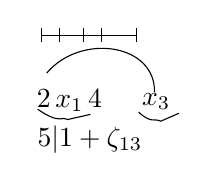
\begin{tikzpicture}[x=.72cm,y=.72cm]
\draw (-.1,1.6)--(1.6,1.6);
\foreach \x in {-.1,.23,.65,.96,1.58}{\draw (\x,1.48)--(\x,1.73);}
\draw (0,.94) .. controls (.6,1.65) and (1.92,1.46) .. (1.9,.6);
\node at (.4,.45) {$\deleted{\unsure{2}}\,x_1\,\deleted{\unsure{4}}$};
\node at (1.93,.44) {$x_3$};
\draw (-.16,.30) .. controls (.25,.02) and (.27,.19) .. (.37,.12) -- (.77,.21);
\draw (1.62,.25) .. controls (1.85,.04) and (1.89,.15) .. (2.01,.09) -- (2.33,.23);
\node at (.76,-.24) {$\unsure{5|1}+\zeta_{13}$};
\end{tikzpicture}}
\figure{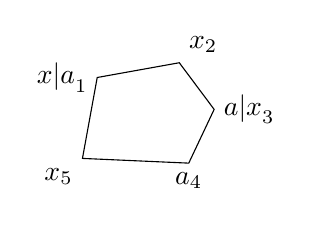
\begin{tikzpicture}[scale=.75]
\draw (-.91,.69)--(.48,.94)--(1.07,.15)--(.64,-.76)--(-1.16,-.68)--cycle;
\node[left] at (-.91,.69) {$\unsure{x|a}_1$};\node[above right] at (.48,.94) {$x_2$};
\node[right] at (1.07,.15) {$\unsure{a|x}_3$};\node[below] at (.64,-.76) {$a_4$};
\node[below left] at (-1.16,-.68) {$x_5$};
\end{tikzpicture}}
\[
\underline{\zeta_{12}}\,\zeta_{34}\,\zeta_{15}\,\underline{\zeta_{23}}\,\zeta_{45}
\qquad 10\,P=720
\]
\[
\deleted{\unsure{46}}\qquad 2\quad2\quad2\quad2\quad2\quad0\qquad P=72
\]
\figure{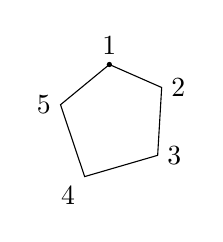
\begin{tikzpicture}[scale=.73]
\draw (0,1)--(.91,.6)--(.84,-.58)--(-.43,-.95)--(-.85,.30)--cycle;
\fill (0,1) circle (1.3pt);
\node[above] at (0,1) {$1$};\node[right] at (.91,.6) {$2$};\node[right] at (.84,-.58) {$3$};\node[below left] at (-.43,-.95) {$4$};\node[left] at (-.85,.30) {$5$};
\end{tikzpicture}}
\[
4!=\qquad
\begin{aligned}P_0&=12\\&=\text{nb \unsure{de|des} struct. pol. sur l'ens à $5$ él}\end{aligned}
\]
\[
\zeta_{i,i+2}\quad\zeta_{j,j+\unsure{2|3}}
\]
\figure{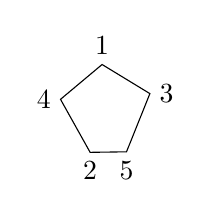
\begin{tikzpicture}[scale=.66]
\draw (0,.96)--(.92,.4)--(.47,-.72)--(-.23,-.73)--(-.8,.29)--cycle;
\node[above] at (0,.96) {$1$};\node[right] at (.92,.4) {$3$};\node[below] at (.47,-.72) {$5$};\node[below] at (-.23,-.73) {$2$};\node[left] at (-.8,.29) {$4$};
\end{tikzpicture}}
% archive sheet number: 44
\scanpage{47}
graphe discret: sans arêtes. Parties discrètes d'un graphe (discrètes pour la structure induite) doublets, triades\inserted{, quadruplets, pentuplets, hextuplets}; parties discrètes de card $2,3$.

\deleted{graphe} graphe \unsure{bi-discret|bidiscret}: graphe \inserted{dont l'ens des sommets} $\Gamma$, décomposé en deux parties discrètes
$A,A'$ $(\Gamma=A\amalg A')$ \deleted{\unsure{avec}} tel que
\deleted{$\forall x\in A\ \exists!x'\in A'$ tel que $\{x,x'\}$}
\inserted{la relation $R$ entre $A,A'$ définie par}
$\{x,x'\}\in R\Longleftrightarrow\{x,x'\}$ est un doublet (i.e. $x,x'$ non liés) est bijective
\unsure{soit|est|sauf} un doublet. Cette décomposition est unique sauf si
$\operatorname{Card} A=2$ \inserted{i.e. $\operatorname{Card}\Gamma=4$} (les graphes de ce dernier type sont \unsure{tous} isom. à
\diagram{\begin{tikzcd}[ampersand replacement=\&,row sep=tiny,column sep=small]
a\arrow[dr,dash]\& b\arrow[dl,dash]\\ a'\& b'
\end{tikzcd}}
$A_2\amalg A_2$, i.e. somme disjointe de deux segments -- et le
choix d'une \deleted{\unsure{A|$\Delta$}} décomposition \inserted{de $\Gamma$} en $A,A'$ équivaut à la donnée d'une bijection entre ces segments.
Bidoublets, bitriades \ldots\ \inserted{biquadruplets, bipentuplets, bihextuples \ldots}
\deleted{parties bi-\unsure{discrètes} d'ordre $n$ (bi}

% slanted
\margin{\uline{NB} les bitriades sont exactement les hexagones}

Dans un graphe cubique, les bases et bibases
sont les \deleted{\unsure{syst\textsuperscript{x}|systèmes} \unsure{parties|$\Gamma=A,A'$}} hextuplets et bihextuplets.

\inserted{Deux parties discrètes \inserted{$A,A'$} d'un graphe sont dites \deleted{``opposées''} ``biliées'' si elles sont disjointes et si leur réunion est \deleted{\unsure{bidiscr.}} un graphe \unsure{(avec ses)} bidiscret pour sa décomposition naturelle.}
% slanted
\margin{elles sont dites liées si elles sont disjointes et si leur réunion est encore discrète. Elles sont dites \uline{opposées} si tt él. de l'une est lié à tt él de l'autre (donc elles sont disjointes)}

\uline{NB} La catégorie des graphes bi-discrets d'ordre $n$ est
l'équivalente canonique à la catégorie $(\mathrm{Ens}_2)\times(\mathrm{Ens})_n$.

Deux triades $\tau=\{a,b,c\}$, $\tau'=\{x,y,z\}$ sont \inserted{donc} \deleted{dites} \uline{liées}
si \deleted{leur réunion} elles sont disjointes et leur réunion
est discrète, (i.e. ssi leur réunion est un hextuplet \unsure{\S} \inserted{ou encore une base.}

\deleted{elles sont dites biliées}

\uline{Proposition} Soit $\Delta=(S,A)$ un graphe cubique, soit
$\mathrm{Tri}_{\Delta}$ l'ens de ses triades, considérons sur $\mathrm{Tri}$, la structure
de graphe définie par la relation des ``triades liées''
précédente. Alors \textcircled{\scriptsize 1} $\mathrm{Tri}$ est \deleted{\unsure{réunion disjointe}} \inserted{un graphe somme} de
\deleted{\unsure{des}} \inserted{\uline{hexagones}} \inserted{(i.e. ses comp. connexes sont des hexagones)}.
\margin{$\operatorname{Card}\mathrm{Tri}_{\Delta}=\unsure{720|{\mathord{?}}20}$}
% slanted
\margin{Hex \unsure{gr.} \deleted{hexagones distingués} des triades: chaque triade appartient à un unique \deleted{hex.} \inserted{hexagone} \deleted{distingué} $\operatorname{Card}\mathrm{Hex}=\unsure{120|720}$}

\textcircled{\scriptsize\unsure{2|1}} Deux triades sont \deleted{biliées} \inserted{opposées au sens plus haut} ssi elles sont sur un $=$ hexagone et \inserted{y} sont \deleted{\unsure{pas liées}} \inserted{opposées} (donc pour tte triade $\exists!$ triade opposée)
\textcircled{\scriptsize 3} Deux triades \inserted{$\tau,\tau'$} sont biliées ssi elles appartiennent à un $=$ \deleted{\unsure{hexagone}} hexagone,
% archive sheet number: 46
\scanpage{48}
et sont ni égales, ni liées, ni opposées, i.e. ssi \inserted{$\tau\ne\tau'$ et} il existe une triade $\tau''$ liée à $\tau$ et $\tau'$.

\textcircled{\scriptsize 4} Soit $\tau$ une triade, soient $\tau',\tau''$ les deux triades liées à $\tau$. Alors
\[
\tau'\amalg\tau''=L(\tau)=\{\text{ens des }s\in S\smallsetminus\tau\text{ liés à aucun }\in\tau\}
\tag*{a)}
\]
\deleted{\unsure{a}} En particulier (compte tenu de \textcircled{\scriptsize 3}) $L(\tau)$ est une bitriade, et $L(\tau)=\tau'\cup\tau''$ est sa décomposition canonique
(ce qui explicite la construction des deux triades $\tau',\tau''$ contigues à une triade $\tau$)

\textcircled{\scriptsize 5} Soit $\bar\tau=E(\tau)$ l'ens des sommets liés à tous les él. de $\tau$. Alors $\bar\tau$ est une triade (donc la triade opposée à $\tau$).
D'où \textcircled{\scriptsize 6} Les deux triades biliées à $\tau$ s'obtient ainsi:
\[
\begin{aligned}
\text{l'une est}\quad&\overline{\tau'}=L(\tau'')\smallsetminus\tau\\
\text{l'autre}\quad&\overline{\tau''}=L(\tau')\smallsetminus\tau
\end{aligned}
\]
\deleted{\textcircled{\scriptsize 7} Les hexagones de triades}
\inserted{L'hexagone} de triades contenant $\tau$ est \deleted{\unsure{$\xi$}}
\[
\tau\ \tau'\ \overline{\tau''}\ \bar\tau\ \overline{\tau'}
\]
(si suivant dans cet ordre circulaire \ldots) \deleted{\unsure{donc}}. Aussi on trouve
\figure{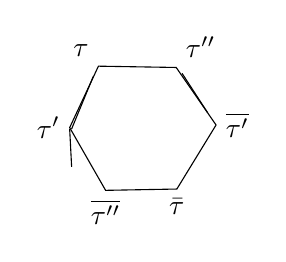
\begin{tikzpicture}[scale=.83]
\draw (-.68,1)--(.51,.98)--(1.12,.1)--(.52,-.88)--(-.57,-.9)--(-1.12,.06)--cycle;
\draw (-1.09,.04)--(-.76,.84) (.60,.89)--(.99,.29) (-1.12,.04)--(-1.09,-.54);
\node[above left] at (-.68,1) {$\tau$}; \node[above right] at (.51,.98) {$\tau''$};
\node[right] at (1.12,.1) {$\overline{\tau'}$}; \node[below] at (.52,-.88) {$\bar\tau$};
\node[below] at (-.57,-.9) {$\overline{\tau''}$}; \node[left] at (-1.12,.06) {$\tau'$};
\end{tikzpicture}}

\textcircled{\scriptsize 7} Pour la relation de ``biliées'', \deleted{\unsure{le graphe|les triades}} \inserted{l'ens} $\mathrm{Tri}$, \deleted{les triades} des triades est un graphe somme de triangles (dits \deleted{triangles triples} \inserted{``triangles} de triades biliées''), dans l'ens des triangles de triades biliées'' \deleted{\unsure{la rel.}} le passage au ``triangle opposé'' est une involution ss pt fixe.
% slanted
\margin{\unsure{Tritria|Tritrio} $={}$ triangle de triades biliées \deleted{est} de cardinal $2\cdot120=240$}
\inserted{les hexagones correspondent aux orbites de cette involution, à tt triangle correspond \unsure{la réunion|l'hexagone} de ce triangle et son opposé.}

\figure{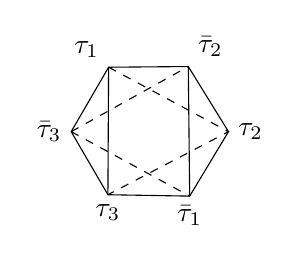
\begin{tikzpicture}[scale=.88]
\draw (-.62,.95)--(.53,.96)--(1.11,.02)--(.55,-.91)--(-.63,-.89)--(-1.16,.02)--cycle;
\draw (-.62,.95)--(-.63,-.89) (.53,.96)--(.55,-.91);
\draw[dashed] (-.62,.95)--(1.11,.02)--(-.63,-.89) (-1.16,.02)--(.53,.96) (-1.16,.02)--(.55,-.91);
\node[above left] at (-.62,.95) {$\tau_1$};\node[above right] at (.53,.96) {$\bar\tau_2$};
\node[right] at (1.11,.02) {$\tau_2$};\node[below] at (.55,-.91) {$\bar\tau_1$};
\node[below] at (-.63,-.89) {$\tau_3$};\node[left] at (-1.16,.02) {$\bar\tau_3$};
\end{tikzpicture}}
\deleted{\textcircled{\scriptsize 8} La réunion (de cardinal $6\cdot3=18$) des triades d'un hexagone a un complémentaire (de cardinal $27-18=9$) qui est un bitriangle. L'application qui à tt hexagone de triades associe \unsure{le} bitriangle précédent, est \uline{bijective}.}
\deleted{les Hexagones \unsure{correspondent}}
% archive sheet number: 47
\scanpage{49}
\textcircled{\scriptsize 8} Soit \deleted{\unsure{$T$}} $\{\tau_i\}_{i\in I}\deleted{\unsure{\{\tau_1,\tau_2,\tau_3\}}}$ un triangle de triades biliées \inserted{(\unsure{noté|noté parfois|noté relation|relation non-liées} \unsure{Natif|Nat.|Notat.})}. \deleted{Alors}
\inserted{soit $I=\{i,j,k\}$,}
\deleted{Soit} Si $x_i\in\tau_i$, et si $x_j$ ($x_k$) est l'unique él. de
$\tau_j$ ($\tau_k$) non lié à $x_i$, alors $x_j$ et $x_k$ sont non liés.

En d'autres termes, si $J\subset\bigl(\prod_{i\in I}\tau_i,\deleted{\unsure{\tau_{i_2},\tau_{i_3}}}\bigr)$ est l'ens des $(x_i)_{i\in I}\deleted{\unsure{(x_j,x_k)}\text{ tels}}$ que $x_i$ non lié à $x_j$ pour $i\ne j$,
alors les projections $J\xrightarrow{\unsure{p_i|\mathrm{Pr}_i}}\tau_i$ sont bijectives (donc on a un syst. transitif d'isom entre les $\tau_i$, via \unsure{$J|t$}).

\deleted{\textcircled{\scriptsize 9} Soit \unsure{$S$ la} $X$ \inserted{$=\tau_1\cup\tau_2\cup\tau_3$} la réunion des trois triades d'un triangle $\{\tau_1,\tau_2,\tau_3\}$ de triades biliées $[\,\bar X=\bar\tau_1\cup\bar\tau_2\cup\bar\tau_3$ la réunion des trois triades du triangle opposé, alors $X,\bar X$ sont de cardinal $9$ et disjoints$]$.}

\textcircled{\scriptsize 9} Soit $X=\coprod_{i\in I}\tau_i\hookrightarrow S$, \inserted{(card $X=9$)} d'où $X\longrightarrow I$, dont les $3$ fibres sont \deleted{des} \inserted{les} \deleted{\unsure{$k$}} $3$ triades du triangle de triades donné:
\deleted{et} Soit $X\longrightarrow J$ l'application dont les restrictions aux $\tau_{\underline i}$ sont les $p_i^{-1}$, \deleted{d'où une application} \inserted{dont les fibres $(\tau'_j)_{j\in J}$ sont des $3$} autres triades \unsure{mutuellt|mutuellement} disjointes. Ceci posé

\textcircled{\scriptsize$\cdot$} $X$ est un bitriangle, \deleted{dont les} \inserted{dont} les six \deleted{\unsure{triades}} \inserted{triades}
(ou antitriangles) sont les $\tau_i$ \deleted{\unsure{$(i)$}} $(i\in I)$ $\tau'_j$ $(j\in J)$. forment les $2$ familles d'\deleted{anti}triades parallèles de $X$. Ainsi
\deleted{L'application $X\to I\times J$ est bijective.}
$I,J$ s'identifient resp. à l'une et l'autre familles de triades du bitriangle $X$, et l'application
\[
 X\longrightarrow I\times J
\]
est bijective.

\textcircled{\scriptsize 10} La donnée d'un triangle de triades biliées $(\tau_i)_{i\in I}$
\uline{équivaut} à celle d'un bitriangle $X$, muni
du \deleted{une} choix d'\uline{une} des deux familles \inserted{$I,J$} de
triades \unsure{mutuellmt|mutuellt|mutuellement} disjointes de $X$ (coorientation)
% archive sheet number: 48
\scanpage{50}
\handwritten{\deleted{\uline{NB} En passant: pour que \unsure{deux|des} triades $\tau_1,\tau_2$ soient biliées, il f et s. qu'elles soient disjointes et appartiennent à un $=$ bitriangle, qui est \unsure{uniquemt|uniquement} déterminé, et est \unsure{aussi|aussitôt} l'unique}}

\handwritten{\textcircled{\scriptsize 11} $X$ est l'unique bitriangle contenant $\tau_i$ -- deux triades sont biliées ssi elles sont \inserted{disjointes et} contenues dans un $=$ bitriangle \deleted{(i.e. \unsure{l})}}

\handwritten{\textcircled{\scriptsize 12} Soit \deleted{\unsure{$X$ ou}} $(\tau_i)_{i\in I}$ un triangle de triades biliées, associé au bitriangle $X=\coprod_{i\in I}\tau_i\subset S$ avec sa coorientation $\{\tau_i\}\deleted{\unsure{\tau_2,\tau_3}}_{i\in I}$, \deleted{soit $(\bar\tau_i)_{i\in I}$ le triangle de} \inserted{$J$ l'ens des} \deleted{\unsure{triades}} \inserted{$(\tau'_j)_{j\in J}$} de $X$ de l'autre famille (de sorte que $X\xrightarrow{\sim}I\times J$). Soit $(\bar\tau_i)_{i\in I}$ le triangle de triades opposé, $\bar X=\bigcup_{i\in I}\bar\tau_i$, et $\bar J$ l'ens des triades de $\bar X$ de l'autre famille, donc $\bar X\xrightarrow{\sim}I\times\bar J$. Soit $\widetilde X=S-X-\bar X$, qui est de cardinal $9$ \inserted{$=27-2\cdot9$}. Alors}

\handwritten{a) $\widetilde X$ est un bitriangle. \deleted{\unsure{Il est|Soit}} L'application qui à tt hexagone de triades associe $\widetilde X$, est bijective. \deleted{\unsure{$S$}}}

% printed form
% Inverted relative to the manuscript. Long diagonal pen strokes cross the form.
\noindent\begin{minipage}[t]{.28\linewidth}
\deleted{Place}\\
\deleted{N\textsuperscript{o}}\par\smallskip

\deleted{UNIVERSITÉ DES SCIENCES ET TECHNIQUES DU LANGUEDOC}

\deleted{(1) -- Le candidat doit indiquer la nature de l'examen auquel il se présente.}

\deleted{(2) -- Le candidat inscrit ses nom, prénom, lieu et date de naissance en tête de la copie et signe lisiblement son nom à la fin de la composition.}

\end{minipage}\hfill\begin{minipage}[t]{.68\linewidth}
\deleted{ACADEMIE DE MONTPELLIER}\par\smallskip

\deleted{Examen de \textsuperscript{(1)}} \dotfill\par
\noindent\dotfill

\deleted{Nom et Prénoms du Candidat \textsuperscript{(2)} \dotfill}

\deleted{né à \dotfill{} département de \dotfill}

\deleted{le \dotfill{} 19}

\deleted{Montpellier, le \dotfill{} 19}

\deleted{COMPOSITION EN} \dotfill
\end{minipage}

% archive sheet number: 49
\scanpage{51}
\deleted{b) L'ens des coorientations de}

b) \deleted{\unsure{$X$ et $\widetilde X$ sont les deux seuls bitriangles disjoints de $X$ et|$X$ et $\widetilde X$ sont les deux seuls bitriangles disjoints de $\bar X$}, \unsure{permutés} \unsure{d'où les trois} symétries}
\inserted{Considérons le groupe $\widetilde G$ d'autom de $X$, \deleted{\unsure{engendré}} engendré par les} symétries $\sigma_t$ $(t\in\mathrm{Tri}(\widetilde X))$. Alors

$\alpha$) $\widetilde G\longrightarrow\mathrm{Aut}_{\unsure{\mathrm{gr}|\mathrm{gr.}}}(\widetilde X)$ \deleted{est} \inserted{induit} un isom. \inserted{de $\widetilde G$} avec le groupe des autom \uline{intérieurs} de $\widetilde X$

$\beta$) Les orbites de $\widetilde G^{\unsure{\circ|0}}$ opérant sur $S-\widetilde X$ $(=X\amalg\bar X^{\unsure{+}})$ sont de cardinal $6$ -- donc il y \deleted{\unsure{en}} a trois telles orbites
\inserted{qui sont les réunions de la forme $\tau\cup\bar\tau$ (triade de l'hexagone \unsure{$H$})}
[On \unsure{a} en effet $\widetilde G\simeq\mathfrak S_{\unsure{P|E|\mathbb F}}\times\mathfrak S_Q$, où $\unsure{\bar P|\widetilde P|\mathbb F},\widetilde Q$ sont les deux ens de card. $3$ des triangles de $\widetilde X$ de l'une et l'autre espèce, \deleted{les orbites sont} $\mathfrak S_P$ et $\mathfrak S_Q$ sont \unsure{simplmt|simplemt|simplement} transitifs sur chacune des trois orbites]
\inserted{Donc l'ens des trois \unsure{orbites|calottes|culottes} s'identifie à l'ens $I$ des $3$ diagonales de $H$.}

c) \deleted{\unsure{$\widetilde G^\circ$ soit le sous-groupe de $\widetilde G$},} \inserted{Si $t\in\mathrm{Tr}(\widetilde X)$}, $\sigma_t$ échange $\tau$ et $\bar\tau$ \unsure{donc|dans} le groupe \inserted{$\widetilde G^\circ\subset\widetilde G$} \deleted{\unsure{engendré}} \inserted{formé par} par les nbrs pairs de symétries \deleted{\unsure{opère}} conserve chacune des $\tau\in H$ -- et les orbites de $\widetilde G^\circ$ sur $S-\widetilde X$ sont de cardinal $3$, et ce sont les $6$ triades de l'hexagone $H$.

\deleted{(Ainsi l'ens des trois \unsure{orb}} \deleted{d) Soit}

\textcircled{\scriptsize 11} \unsure{Soit|Soient} $(X_\alpha)_{\alpha\in A}$ une famille de trois bitriangles mutuellmt disjoints. Pour $\alpha\in A$, soit $I_\alpha$ l'ens de cardinal $3$ associé à $X_\alpha$ (\deleted{des} \inserted{l'ens} trois orbites de $\mathrm{AutInt}(X_\alpha)$ opérant sur $S-X_\alpha=\bigcup_{\beta\in A-\{\alpha\}}X_\beta$ On a donc une application $X_\beta\xrightarrow{p_{\alpha\beta}}I_\alpha$ $(\beta\ne\alpha)$
% archive sheet number: 50
\scanpage{52}
\deleted{\unsure{dont}} de degré $3$, dont les \inserted{$3$} fibres sont les \inserted{trois} triades (\unsure{mutuellmt|mutuellt|mutuellement} disjointes) formant l'une des deux familles de triades de $X_\beta$. Alors

a) Les \deleted{\unsure{autres}} deux familles de triades, fibres des deux applications $X_\alpha\to I_\beta$, $X_\alpha\unsure{-|\to}I_\gamma$ (où \deleted{\unsure{$\alpha$}} $A=\{\alpha,\beta,\gamma\}$) sont distinctes, donc l'application correspondante $X_\alpha\xrightarrow{\sim}I_\beta\times I_\gamma$ est bijective.

Plus intrinsèquemt, $\forall\alpha\in A$, on a
\[
 X_\alpha\xrightarrow{\sim}\prod_{\beta\in I-\{\alpha\}} I_\beta
\]
d'où une bijection naturelle
\[
 S\simeq\coprod_\alpha\prod_{\beta\in I-\{\alpha\}}I_\beta\quad\deleted{\unsure{I_{\alpha}}}
\]
dans le cas où $A=\{1,2,3\}$, cela fait
\[
 S\simeq\underbrace{I_2\times I_3}_{X_1}\ \amalg\
 \underbrace{I_3\times I_1}_{X_2}\ \amalg\
 \underbrace{I_1\times I_2}_{X_3}
\]
On a $\mathrm{coor}(X_\alpha)\simeq\deleted{\unsure{I_\alpha}}A-\{\alpha\}$.

c) Pour que \deleted{$x_\alpha\in X_\alpha,y_\alpha\in$ \unsure{avec} $\unsure{x\ne y}$} $x_\alpha,y_\alpha\in X_\alpha$ \deleted{$\unsure{x_\alpha\ne y_\alpha}$}, soient \uline{non liés} il f. et s. que $\exists\beta\in A-\{\unsure{\alpha|\beta}\}$ \deleted{\unsure{que}} tel que $p_{\beta\alpha}(x_\alpha)=p_\beta(y_\alpha)$ (si $x_\alpha\ne y_\alpha$, ce $\beta$ est unique) -- pour qu'ils soient liés, il f et s. que $\forall\beta\in A-\{\alpha\}$, on ait $p_{\beta\alpha}(x_\alpha)\ne p_{\beta\alpha}(y_\alpha)$

d) Pour que $x_\alpha\in X_\alpha$ et $y_\beta\in X_\beta$ $(\alpha\ne\beta)$ soient liés il f et s que (si $\gamma$ \deleted{tel que} est l'élémt $\ne\alpha,\beta$ de $A$) on ait $p_{\gamma\alpha}(x_\alpha)=p_{\gamma\beta}(x_\beta)$
% archive sheet number: 51
\scanpage{53}
\diagram{\begin{tikzcd}[ampersand replacement=\&,column sep=small]
 I\arrow[d,"p"] \& I_\alpha\\ A \& \alpha
\end{tikzcd}}
$S\simeq$ ens des parties \inserted{$\deleted{\unsure{I}}A$} de cardinal $2$ de $I$, telles que $p|A$ soit injectif. (sections partielles sur parties de cardinal $2$)

\figure{\begin{tikzpicture}[scale=.44]
\foreach \x in {0,1,2}{\foreach \y in {1.5,2.5,3.5}{\fill (\x,\y) circle (.042);}\fill (\x,0) circle (.065);}
\draw[line width=1.6pt] (0,3.5)--(1,2.5);
\draw[->] (2.75,1.2)--(2.75,.34);
\end{tikzpicture}}
$X_\alpha=$ ens des $A$ tels que $p(A)=A-\{\alpha\}$

$A,B\in S$ liés ssi $A\ne B$ et
\[
\begin{aligned}
 &\text{ou bien }p(A)=p(B)\qquad A\cap B=\varnothing\\
 &\text{ou bien }p(A)\ne p(B),\quad A\cap B\ne\varnothing
\end{aligned}
\]

\textcircled{\scriptsize 12} La catégorie des graphes cubiques, munis d'une décomposition en trois \deleted{\unsure{bistriangles|bistriples|bitriangles}} \inserted{bitriangles} disjoints, est équivalente à \deleted{celle} \inserted{la cat. $(\mathrm{Ens})_{(3,3,3)}$} des ens \deleted{de type} munis d'une partition de type $(3,3,3)$. Le groupe des autom d'une telle structure est $\simeq\mathfrak S_3\mathbin{.}(\mathfrak S_3\times\mathfrak S_3\times\mathfrak S_3)$ qui est d'ordre $3^4\,2^4$ (c'est donc \inserted{presque} un sous-groupe de Sylow de $\mathrm{Aut}(\Delta)\deleted{\unsure{\ne2}}$ !)
\inserted{il faut se donner des \deleted{\unsure{orientations}} \inserted{\unsure{ordres|cycles|cinq} circ.} des $I_\alpha$ et de $A$ et exiger qu'ils soient respectés \ldots}

% slanted
\margin{\uline{NB} La \deleted{\unsure{réunion|réunition}} \inserted{partition} de $S$ en les $X_\alpha$ se reconstitue, à partir de ce ss-gpe de $\mathrm{Aut}(\Delta)$, comme l'ens des $3$ orbites sur $S$ de ce gpe: donc ce ss-gpe de Sylow est son propre normalisateur.}

La cat. des couples $(\Delta,X)$ d'un graphe cubique, et d'un bitriangle $X$ dans $\Delta$, est équivalente à \deleted{celle des} \inserted{la cat.} \deleted{couples} $(\mathrm{Ens})_3\times(\mathrm{Ens})_{3,3}$ des couples formés d'un ens de card. $3$ (savoir l'ens \deleted{\unsure{des élémts}} \inserted{can. de} \unsure{$P$|$P$ de} orbites associé à $X$ dans $\Delta$) et d'un ens à partition de type $(3,3)$ (savoir l'ens des triades de $X$, \deleted{\unsure{\}|)}} avec sa partition naturelle).
% archive sheet number: 52
\scanpage{54}
\textcircled{\scriptsize 13} L'ens des $18$ triades de $S$ contenues dans un des $X_\alpha$ est en corr. biunivoque avec \deleted{l'ens} le sous-ens $T$ de $I\times A$ formé des couples $(i,\alpha)$ avec $p(i)\ne\alpha$, en associant à un tel couple la triade \inserted{$\tau_{i,\alpha}\subset X_\alpha$} formée des $A\in S\subset\mathcal P_2(I)$ tels que $p(A)=\Lambda-\{\alpha\}$, $A\ni i$. \deleted{\unsure{dira|distincts} $\unsure{\tau_{i,\alpha}\subset}$} La triade opposée à $\tau_{i\alpha}$ est $\tau_{i,\deleted{\unsure{\beta}}\beta'}$, où \deleted{\unsure{$\beta$ est l'él.}} \inserted{$\beta'$} \inserted{l'autre} él. de \deleted{\unsure{$A$|$\Lambda$}} $A-\{p(i)\}$. Les deux triades \deleted{\unsure{bi}}liées à $\tau_{i,\alpha}$ sont $\tau_{j,\unsure{\beta'|\beta}},\tau_{k,\unsure{\beta'|\beta}}$, où $j,k$ sont les \inserted{2 autres} élémts de \deleted{$p^{-1}(p(i))$} $I$ au dessus de $p(i)$. Les deux triades \uline{biliées} à $\tau_{i,\alpha}$ sont $\tau_{j,\beta}\deleted{\unsure{\alpha}},\tau_{k,\beta}$. L'hexagone formé de ces six triades est formé de l'ens des $\tau_{i,\alpha}$ tels que $p(i)=r$ soit donné. L'ens de ces hex. est donc en corr. $1$-$1$ avec $A$ [$:$ l'hexagone $H$ correspondent le complémentaire de sa réunion dans $S$]

\figure{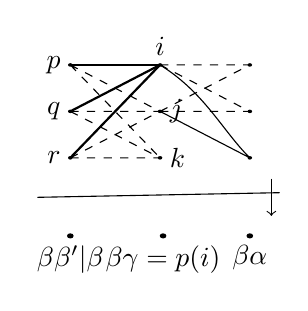
\begin{tikzpicture}[x=.76cm,y=.59cm]
\foreach \x in {0,1.5,3}{\foreach \y in {0,1,2}{\fill (\x,\y) circle (.038);}}
\foreach \y in {0,1,2}{\draw[thick] (0,\y)--(1.5,2);}
\draw[dashed] (0,2)--(1.5,1) (0,2)--(1.5,0) (0,1)--(1.5,1) (0,1)--(1.5,0) (0,0)--(1.5,0) (0,0)--(1.5,1);
\draw[dashed] (1.5,2)--(3,2) (1.5,2)--(3,1) (1.5,1)--(3,1) (1.5,1)--(3,2);
\draw (1.5,2) .. controls (2.25,1.4) and (2.55,.57) .. (3,0) (1.5,1)--(3,0);
\node[left] at (0,2) {$p$};\node[left] at (0,1) {$q$};\node[left] at (0,0) {$r$};
\node[above] at (1.5,2) {$i$};\node[right] at (1.5,1) {$j$};\node[right] at (1.5,0) {$k$};
\draw (-.55,-.85)--(3.5,-.75);\draw[->] (3.36,-.45)--(3.36,-1.25);
\foreach \x in {0,1.55,3}{\fill (\x,-1.68) circle (.056);}
\node[below] at (0,-1.68) {$\deleted{\unsure{\beta}}\unsure{\beta'|\beta}$};
\node[below] at (1.55,-1.68) {$\deleted{\unsure{\beta}}\unsure{\gamma}=p(i)$};
\node[below] at (3,-1.68) {$\deleted{\unsure{\beta}}\alpha$};
\end{tikzpicture}}

\deleted{\textcircled{\scriptsize 14} L'ens \inserted{à $6$ él.} des couples formés d'un des \deleted{\unsure{2}} bitriangles $X_\alpha$, et d'une \uline{coorientation} de $X_\alpha$, est $\simeq$ l'ens des \deleted{\unsure{couples}} couples $(\alpha,\beta)\in A^2$ \deleted{\unsure{ou}} avec $\beta\ne\alpha$ (i.e. à l'ens des repères $(\alpha,\beta,\gamma)$ de l'ens $A$ de cardinal $3$), à $(\alpha,\beta)$ correspond le}
% archive sheet number: 53
\scanpage{55}
le couple $\bigl(X_\alpha,\{\tau_{i,}$
% archive sheet number: 54
